\title{Residuals and Least-Squares}
\subtitle{\SubTitleName}
\institute[]{\Course}
\author{\Instructor}
\maketitle   


\begin{frame}\frametitle{Topics and Objectives}
    \Emph{Topics} \\
    %\TopicStatement
    \begin{itemize}
    
        \item residuals and the residual vector
        % \item mean-deviation form
        
    \end{itemize}
    
    \vspace{0.5cm}
    
    \Emph{Learning Objectives}\\
    
    \begin{itemize}
    
        \item characterize how well a linear model of the form $y = c_0 + c_1 x$ fits given data
        % \item apply mean-deviation form to a linear model
      
    \end{itemize}
    
    \vspace{0.25cm} 
 
\end{frame}
 
 
 


 



\begin{frame}
\frametitle{Motivation}

    \begin{itemize}
        \item<2-> linear models are commonly used in science and engineering model relationships between two or more quantities $\Rightarrow$ knowing more about this process is likely to be of use to many students
        
        \item<3-> a better understanding of what the least-squares method is doing will aid in our understanding of how to interpret results from our algorithms, and determine which algorithms to use
        
        \item<4-> to this end, in this video we will introduce the \Emph{residual vector} to characterize how well our model fits the data
        
    \end{itemize}

\end{frame}


\begin{frame}
\frametitle{Example: Linear Model of the Form $y = c_0 + c_1x$}

    Suppose we are given the data below. 
    \begin{center}
    \begin{tabular}{c|cccc} 
    $ x_i$ & 2 & 5 & 7 & 8 
    \\ \hline 
    $ y_i$ & 1 & 1 & 4 & 3 
    \end{tabular}
    \end{center}
    
    We wish to identify $c_0$ and $c_1$ so that $ y= c_0 + c_1 x$ best fits the data.
    
    \vspace{6pt}
    
    \pause
    The graph below shows our data. 
    \begin{center}
     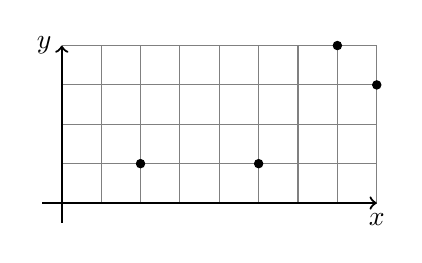
\begin{tikzpicture}[scale=0.5]
        \draw[gray,step=1cm,] (0,0) grid (8,4); 
        \draw[->,thick]  (-.5,0) -- (8,0)  node [below] {$ x$}; \draw[->,thick]  (0,-.5) -- (0,4) node [left] {$ y$}; 
    % \draw[-,very thick, Teal] (0,-0.2) --  (8,3.4); 
    \foreach \x/\y in  {2/1, 5/1, 7/4 , 8/3}  \filldraw (\x,\y) circle (.3em);  
    % \draw[-,DarkRed,thick] (2,1) -- (2,0.66);
    % \draw[-,DarkRed,thick] (5,1) -- (5,2.02);
    % \draw[-,DarkRed,thick] (7,4) -- (7,2.93);
    % \draw[-,DarkRed,thick] (8,3) -- (8,3.4);
    %\foreach \x/\y in  {2/1, 5/2, 7/3 , 8/3} \draw [red,thick] (\x,\y) -- (\x,.45\y-0.23);  
    \end{tikzpicture}
    
    Do you think the values of $c_0$ and $c_1$ will be positive? Negative? 
    
    \end{center} 

\end{frame}
 
 
\begin{frame}
\frametitle{Example: Linear Model of the Form $y = c_0 + c_1x$}

    Compute the equation of the line $ y= c_0 + c_1 x$ that best fits the data 
    
    \begin{center}
    \begin{tabular}{c|cccc} 
    $ x$ & 2 & 5 & 7 & 8 
    \\ \hline 
    $ y$ & 1 & 1 & 4 & 3 
    \end{tabular}
    \end{center}
    
    
    \pause
    To solve this problem, we might construct the system
    \begin{equation*}
    \begin{pmatrix}
    1 & 2 \\ 1 & 5 \\ 1 & 7 \\ 1 & 8 
    \end{pmatrix} \begin{pmatrix}
    c _0 \\ c _1 
    \end{pmatrix} = \begin{pmatrix}
    1 \\ 1 \\ 4 \\ 3 
    \end{pmatrix}
    \end{equation*}
    This is a least-squares problem :   $ A \vec x = \vec y$. We can solve this using the normal equations directly, or with a QR decomposition. 
    
\end{frame}
 
 
 




\begin{frame}{Solution using Normal Equations}
If we use the normal equations directly, we have 
\begin{align*}
A ^{T} A = \begin{pmatrix} 4 & 22 \\ 22 & 142 \end{pmatrix} , \qquad 
A ^{T} \vec y = \begin{pmatrix} 9 \\ 59 \end{pmatrix}
\end{align*}

The least-squares solution is given by solving
\begin{equation*}
\begin{pmatrix}4 &22 \\  22 & 142 \end{pmatrix} \begin{pmatrix} c_0 \\ c_1 \end{pmatrix} = \begin{pmatrix} 9 \\ 59 \end{pmatrix}
\end{equation*}

After solving this linear system, we obtain $c_0 = -5/21$ and $c_1 = 19/42$. 
\begin{equation*}
    y = c _0 + c _1 x = \frac{-5}{21} + \frac{19}{42} x 
\end{equation*}

As we may have guessed, $c_0$ is negative, and $c_1$ is positive.
\end{frame}


\begin{frame}
\frametitle{Questions}

    Looking back at this process, we ask the following questions. 
    \begin{enumerate}
        \item <2-> How well does our model approximate the given data? 
        \item <3-> How can we characterize the degree to which our model fit our data? 
    \end{enumerate}
\end{frame}


\begin{frame}
\frametitle{Model Fit}
    
    Using our model, $$\widehat y_i = c_0 + c_1 x_i = \frac{-5}{21} + \frac{19}{42} x_i$$ we obtain four estimates, $\widehat y_i$.  
    \onslide<2->{
        \begin{center}
            \begin{tabular}{c|cccc} 
            $ x_i$ & 2 & 5 & 7 & 8 
            \\ \hline 
            $ y_i$ & 1 & 1 & 4 & 3  \\ \hline
            $\widehat y_i$ & 0.67 & 2.02 & 2.93 & 3.38
            \end{tabular}
        \end{center}
    }

\end{frame}


\begin{frame}
\frametitle{Model Fit}
    \onslide<1->{Our straight line, $y_i$, and $\widehat y_i$ are shown below.} 
    
    \begin{center}
    
    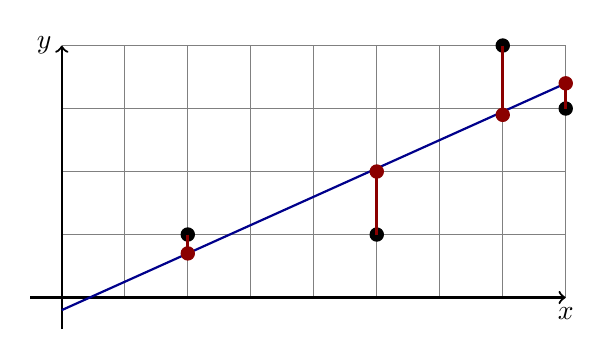
\begin{tikzpicture}[scale=0.8]
            \onslide<2->{ 
            \draw[gray,step=1cm,] (0,0) grid (8,4); 
            \draw[->,thick]  (-.5,0) -- (8,0)  node [below] {$ x$}; \draw[->,thick]  (0,-.5) -- (0,4) node [left] {$ y$}; 
            \draw[-, thick, DarkBlue] (0,-0.2) --  (8,3.4); 
            \foreach \x/\y in  {2/1, 5/1, 7/4 , 8/3}  \filldraw (\x,\y) circle (.3em); 
            \foreach \x/\y in  {2/0.7, 5/2, 7/2.9 , 8/3.4}  \filldraw[DarkRed] (\x,\y) circle (.3em);  
            \onslide<4->{
            \draw[-,DarkRed,very thick] (2,1) -- (2,0.66);
            \draw[-,DarkRed,very thick] (5,1) -- (5,2.02);
            \draw[-,DarkRed,very thick] (7,4) -- (7,2.93);
            \draw[-,DarkRed,very thick] (8,3) -- (8,3.4);
            }            
            }
    \end{tikzpicture}
    
    \onslide<3->{Can we use the distance between the data and our straight line to describe how well our model fit the data?  }

    \end{center} 

\end{frame}



\begin{frame}
\frametitle{Residuals}

\onslide<2->{By using the normal equations, we found the $\vec x$ that minimized }
$$\onslide<2->{\lVert A\vec x - \vec y \rVert }$$
\onslide<3->{over all possible $\vec x \in \mathbb R^n$. This is equivalent to minimizing $$\lVert A\vec x - \vec y \rVert^2 $$ over all possible $\vec x \in \mathbb R^n$.} \onslide<4->{Now let $\vec r = A \vec x- \vec y$. Then,}
\begin{align*}
    \onslide<5->{\lVert A\vec x - \vec y \rVert^2 &= \lVert \vec r \rVert^2 } \onslide<6->{= \sum_{i=1}^n r_i^2}
\end{align*}
\onslide<6->{Where $r_i$ are the entries of $\vec r$. } \onslide<7->{$\vec r$ is the \Emph{residual vector}, and $r_i$ are the \Emph{residuals}.}

% What are we trying to do?  \onslide<2->{Recall that }
% \begin{align*}
%     \onslide<2->{\widehat x & \text{ is the least-squares solution to} A\vec x = \vec b} \\
%     \onslide<3->{A\widehat x = \widehat y & \text{ is the closest vector in } \Col A \text{ to } \vec y }
%     \end{align*}


\end{frame}





\begin{frame}
\frametitle{Least-Squares Optimization}

     \onslide<2->{Our goal with least-squares is to minimize $$\lVert \vec r \rVert^2 = \sum_{i=1}^n r_i^2$$}
    
    \onslide<3->{Our previous example led to the linear model below.} 
    
    \begin{center}
    
    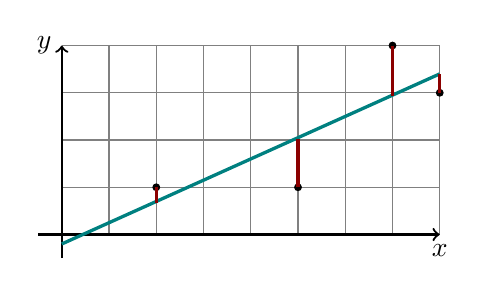
\begin{tikzpicture}[scale=0.6]
            \onslide<4->{ 
            \draw[gray,step=1cm,] (0,0) grid (8,4); 
            \draw[->,thick]  (-.5,0) -- (8,0)  node [below] {$ x$}; \draw[->,thick]  (0,-.5) -- (0,4) node [left] {$ y$}; 
            \draw[-,very thick, Teal] (0,-0.2) --  (8,3.4); 
            \foreach \x/\y in  {2/1, 5/1, 7/4 , 8/3}  \filldraw (\x,\y) circle (.2em);  
            }
            \onslide<5->{
            \draw[-,DarkRed,very thick] (2,1) -- (2,0.66);
            \draw[-,DarkRed,very thick] (5,1) -- (5,2.02);
            \draw[-,DarkRed,very thick] (7,4) -- (7,2.93);
            \draw[-,DarkRed,very thick] (8,3) -- (8,3.4);
            }
    \end{tikzpicture}
    
    \onslide<6->{
    The least-squares line minimizes the sum of squares of the residuals.  }

    \end{center} 


\end{frame}





\begin{frame}
\frametitle{The Distance Between $\vec y$ and $\Col A$ is $||\vec r||$}

    \begin{itemize}
        \item<1-> As we are trying to minimize $\lVert \vec r \rVert^2$.
        \item<2-> Note that $\lVert \vec r \rVert^2 $ is the squared distance between $\vec y$ and $\Col A$. 
        \item<3-> In our example, this is: 
        $$\lVert \vec r \rVert^2 = \lVert \widehat y - \vec y \rVert^2, \quad \vec r = \spalignmat{.67;2.02;2.93;3.38} - \spalignmat{1;1;4;3}= \spalignmat{-0.33;1.02;1.07;0.38}$$
    \end{itemize}
    \onslide<4->{
    We can calculate that $||\vec r||^2 \approx 2.44$. This is a way of describing how well our model fits our data. 
    }
\end{frame}



 \frame{\frametitle{Summary}

    \SummaryLine \vspace{4pt}
    \begin{itemize}\setlength{\itemsep}{8pt}

        \item characterizing how well a linear model of the form $y = c_0 + c_1 x$ fits given data by using residuals and the residual vector

    \end{itemize}
    
    \vspace{16pt}
    \pause 
    
    
}
